\documentclass[xetex,mathserif,serif]{beamer}
\usepackage{polyglossia}
\setdefaultlanguage[babelshorthands=true]{russian}
\usepackage{minted}
\usepackage{tabu}

\useoutertheme{infolines}

\usepackage{fontspec}
\setmainfont{FreeSans}
\newfontfamily{\russianfonttt}{FreeSans}

\definecolor{links}{HTML}{2A1B81}
\hypersetup{colorlinks,linkcolor=,urlcolor=links}

\usepackage{forest}
\usetikzlibrary{arrows}

\tabulinesep=0.7mm

\newcommand{\attribution}[1] {
    \vspace{-5mm}\begin{flushright}\begin{scriptsize}\textcolor{gray}{\textcopyright\, #1}\end{scriptsize}\end{flushright}
}

\title{Системы контроля версий, git}
\author[Юрий Литвинов]{Юрий Литвинов \newline \textcolor{gray}{\small\texttt{y.litvinov@spbu.ru}}}

\date{21.09.2021}

\begin{document}
    
    \frame{\titlepage}
    
    \begin{frame}
        \frametitle{Мотивация}
        \begin{itemize}
            \item Откат изменений
            \item Управление версиями
            \item Централизованное хранение кода
            \item Командная разработка
        \end{itemize}
    \end{frame}

    \begin{frame}
        \frametitle{Локальные копии}
        \begin{center}
            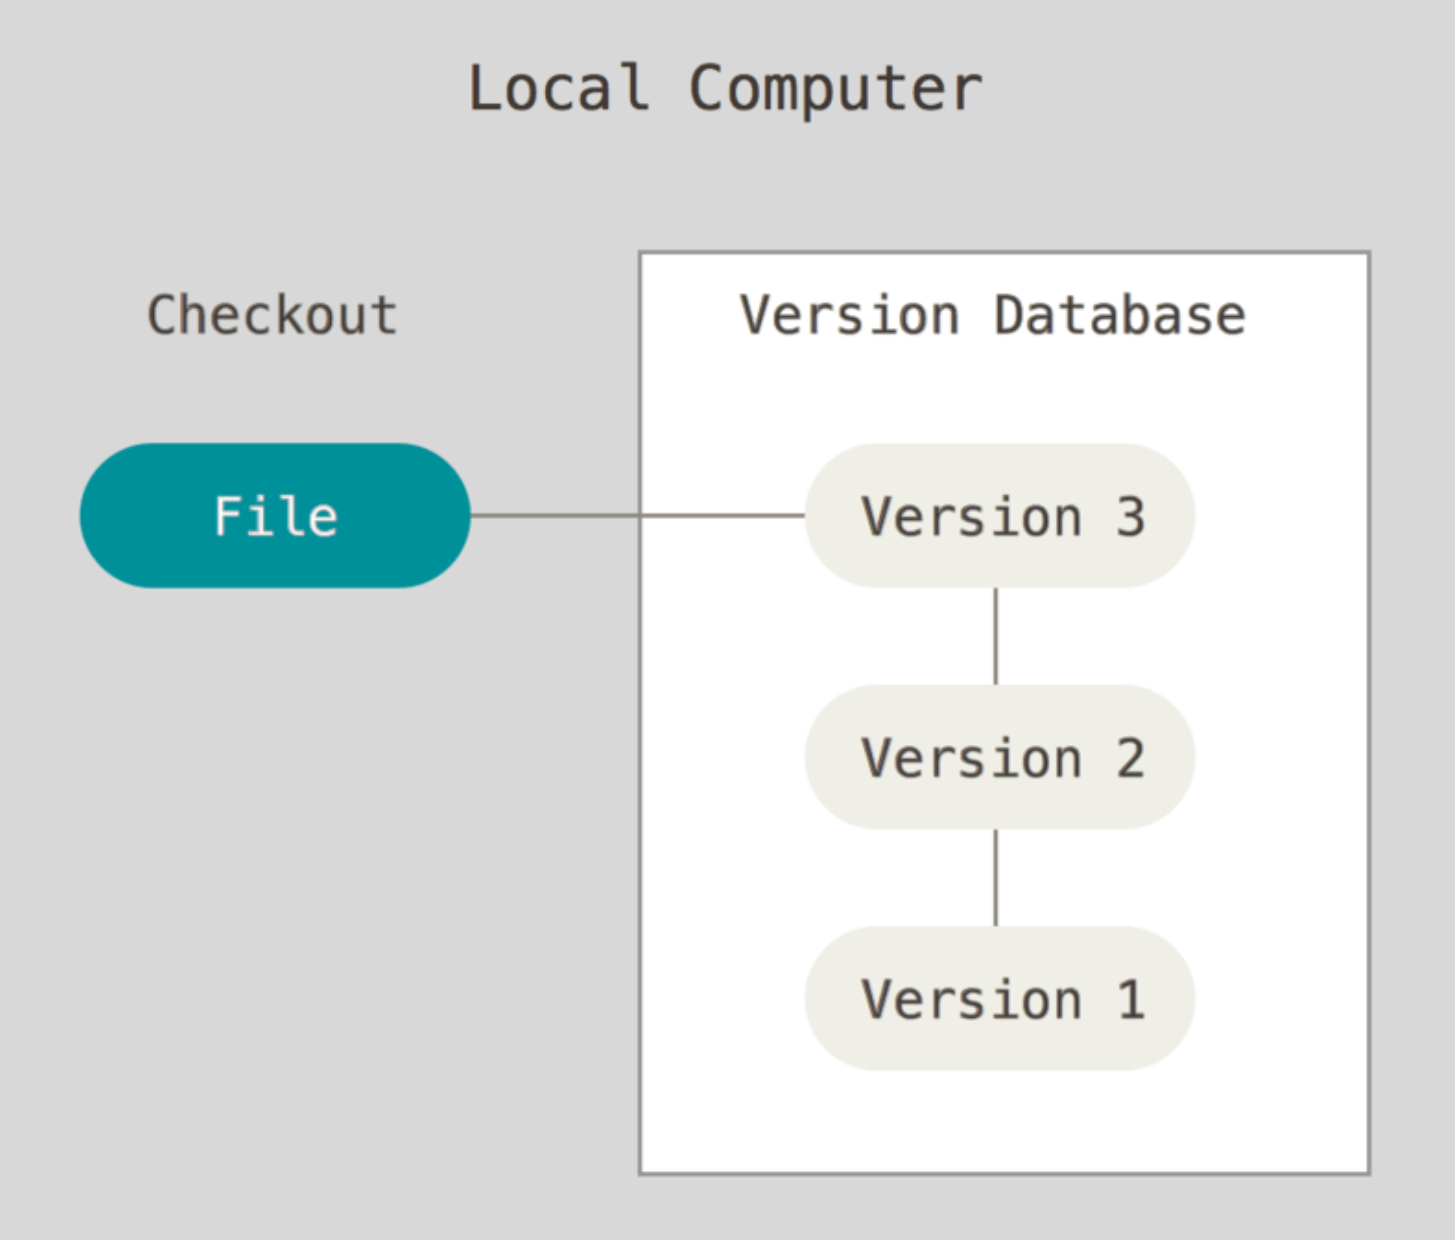
\includegraphics[width=0.6\textwidth]{localCopies.png}
            \attribution{https://git-scm.com/book/ru}
        \end{center}
    \end{frame}

    \begin{frame}
        \frametitle{Централизованные VCS}
        \begin{center}
            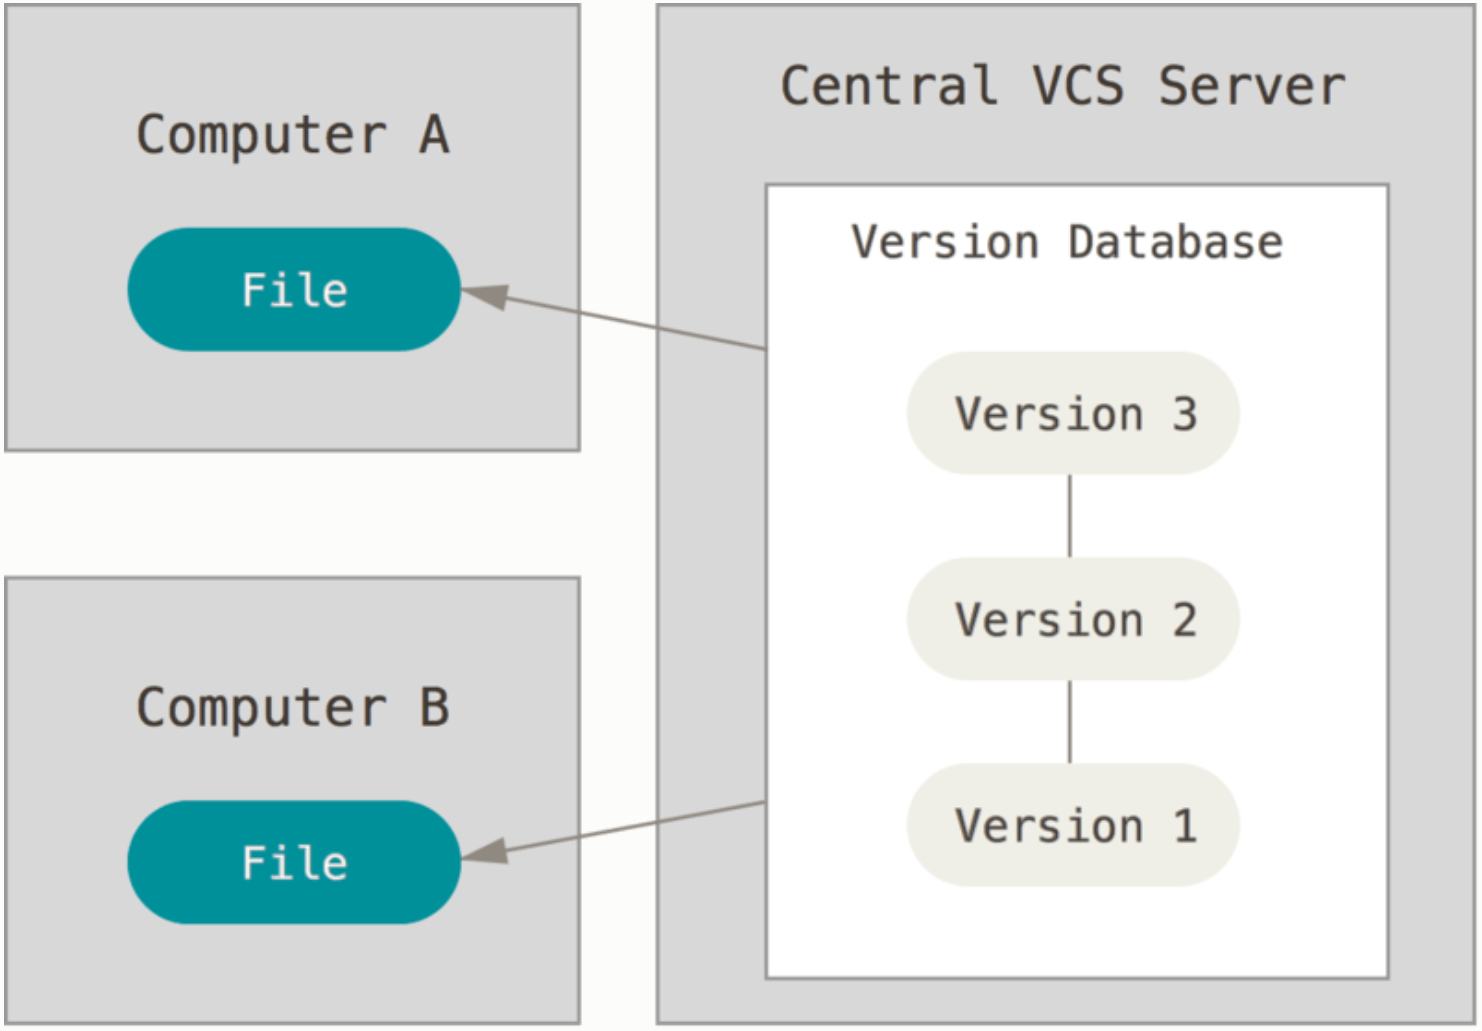
\includegraphics[width=0.6\textwidth]{centralizedVcs.png}
            \attribution{https://git-scm.com/book/ru}
        \end{center}
    \end{frame}

    \begin{frame}
        \frametitle{Распределённые VCS}
        \begin{center}
            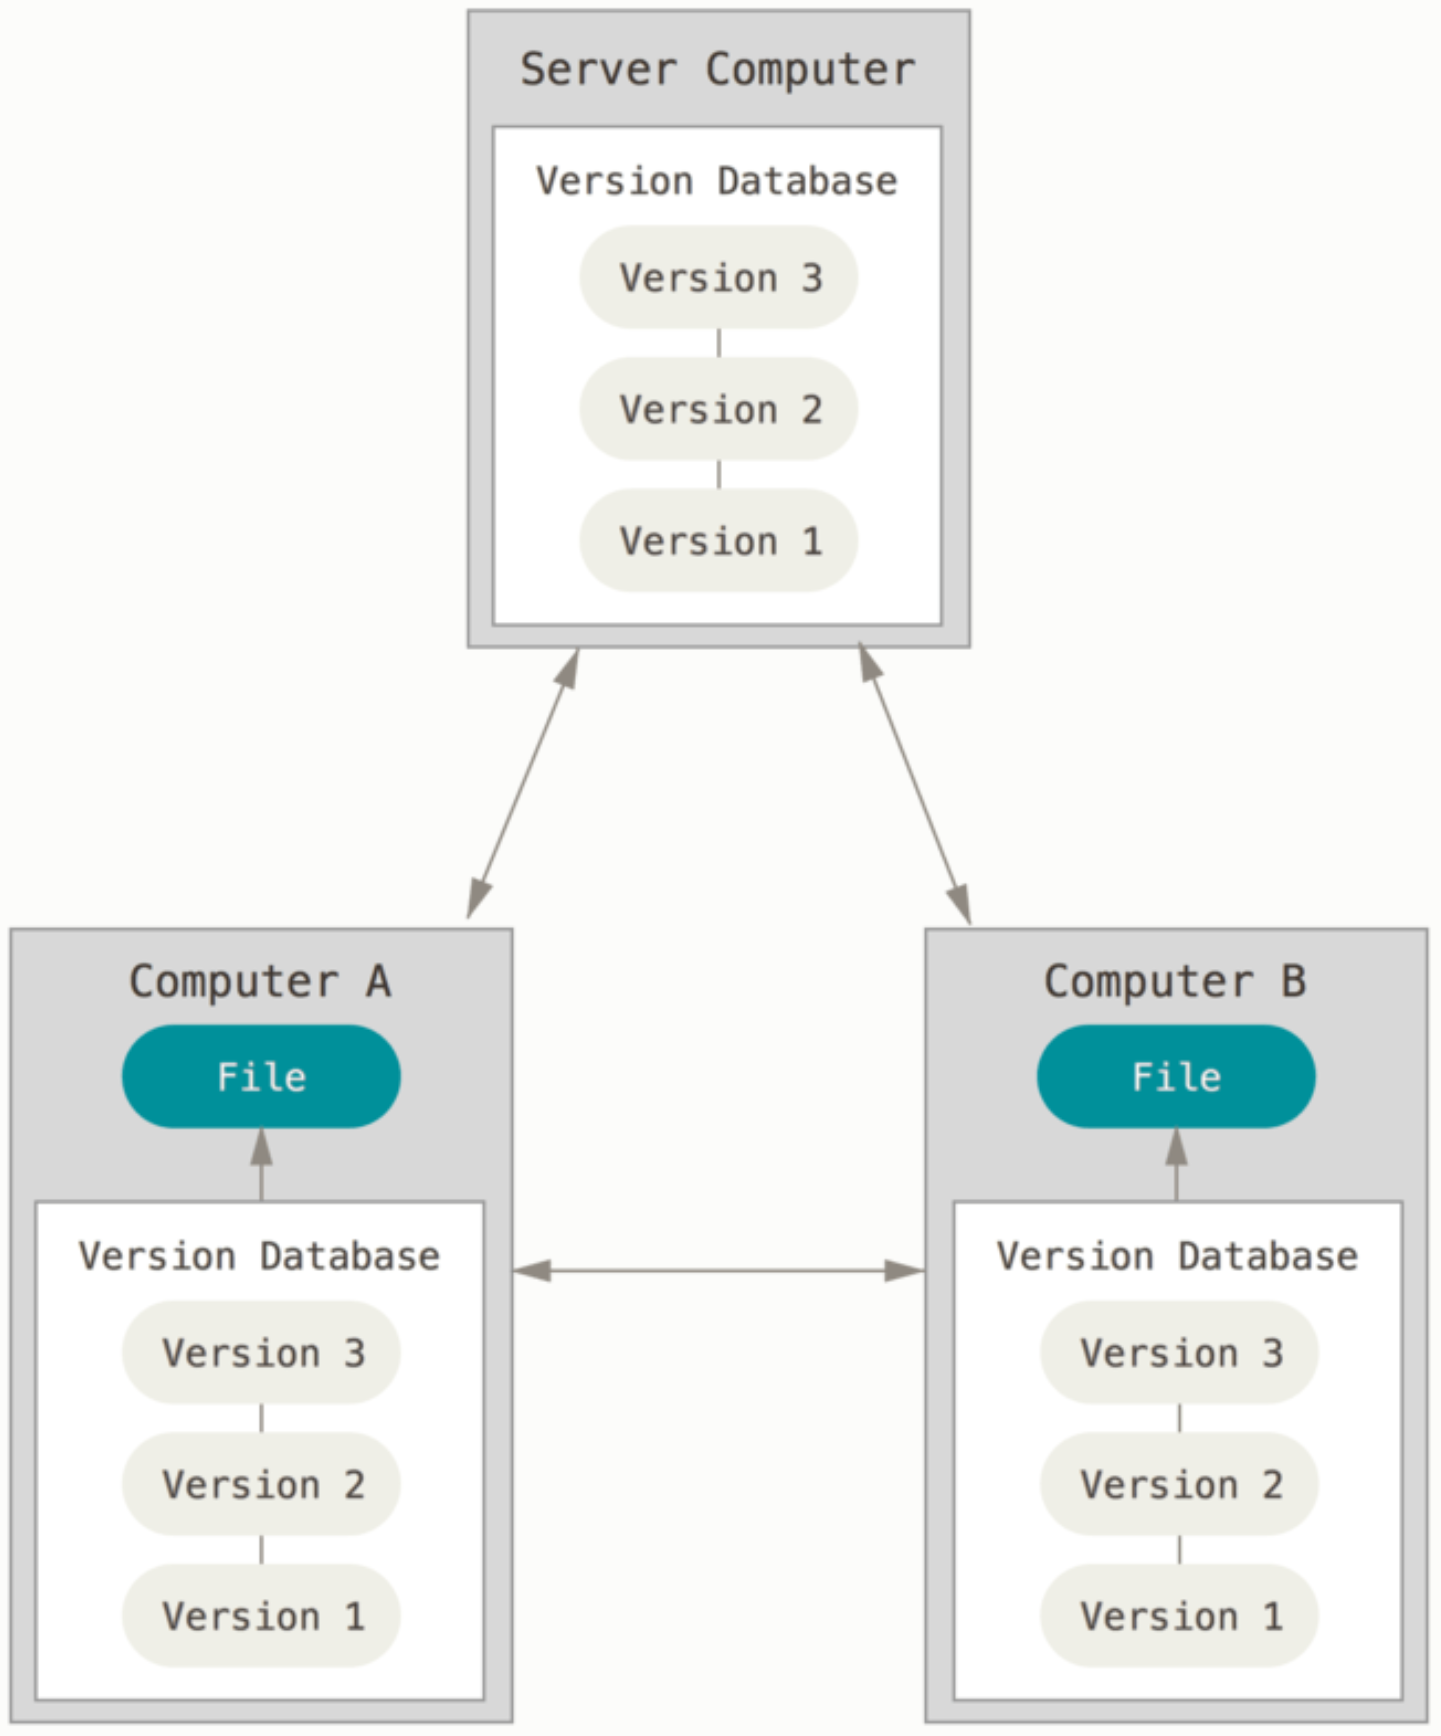
\includegraphics[width=0.4\textwidth]{distributedVcs.png}
            \attribution{https://git-scm.com/book/ru}
        \end{center}
    \end{frame}

    \begin{frame}
        \frametitle{Управление версиями}
        \begin{center}
            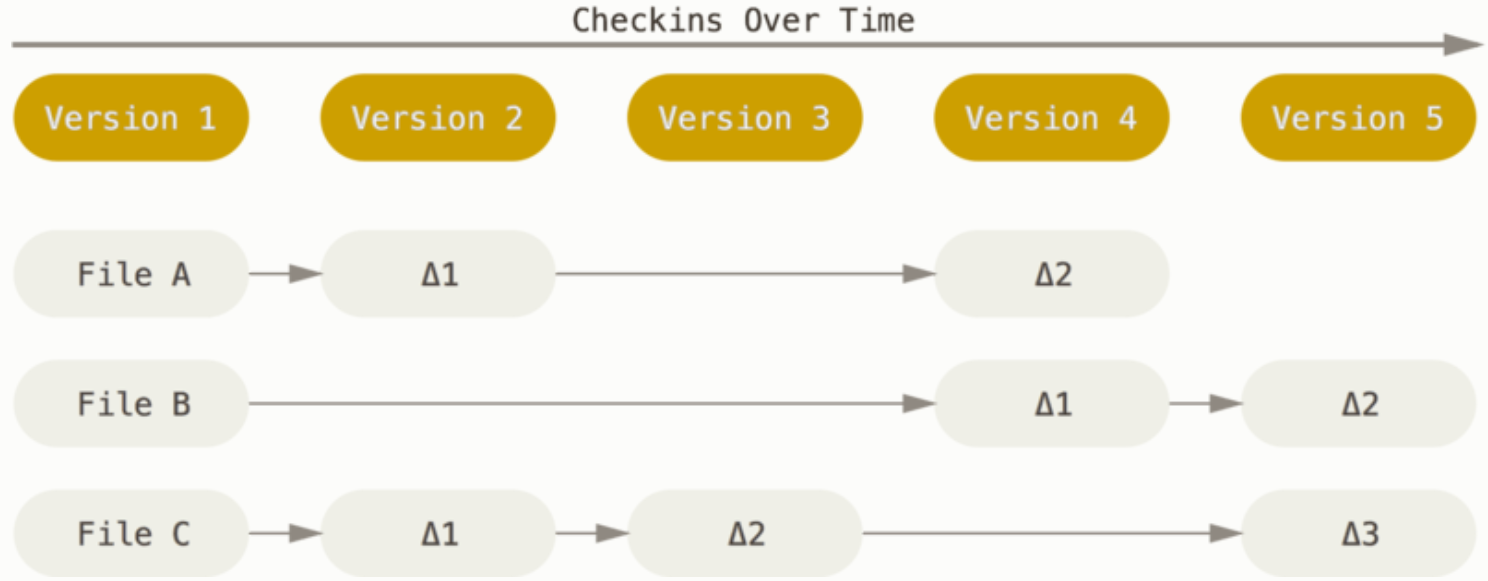
\includegraphics[width=0.6\textwidth]{deltaVersioning.png}

            \vspace{5mm}
            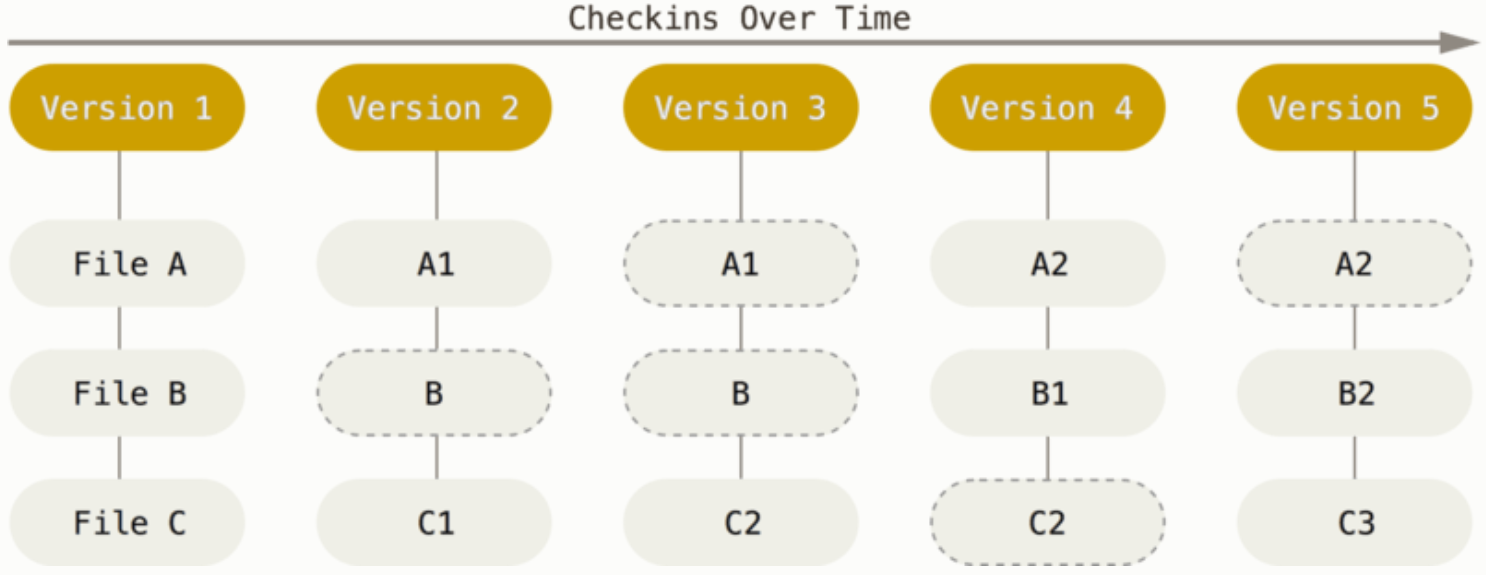
\includegraphics[width=0.6\textwidth]{snapshotVersioning.png}
            \attribution{https://git-scm.com/book/ru}
        \end{center}
    \end{frame}

    \begin{frame}
        \frametitle{Дельта}
        \begin{center}
            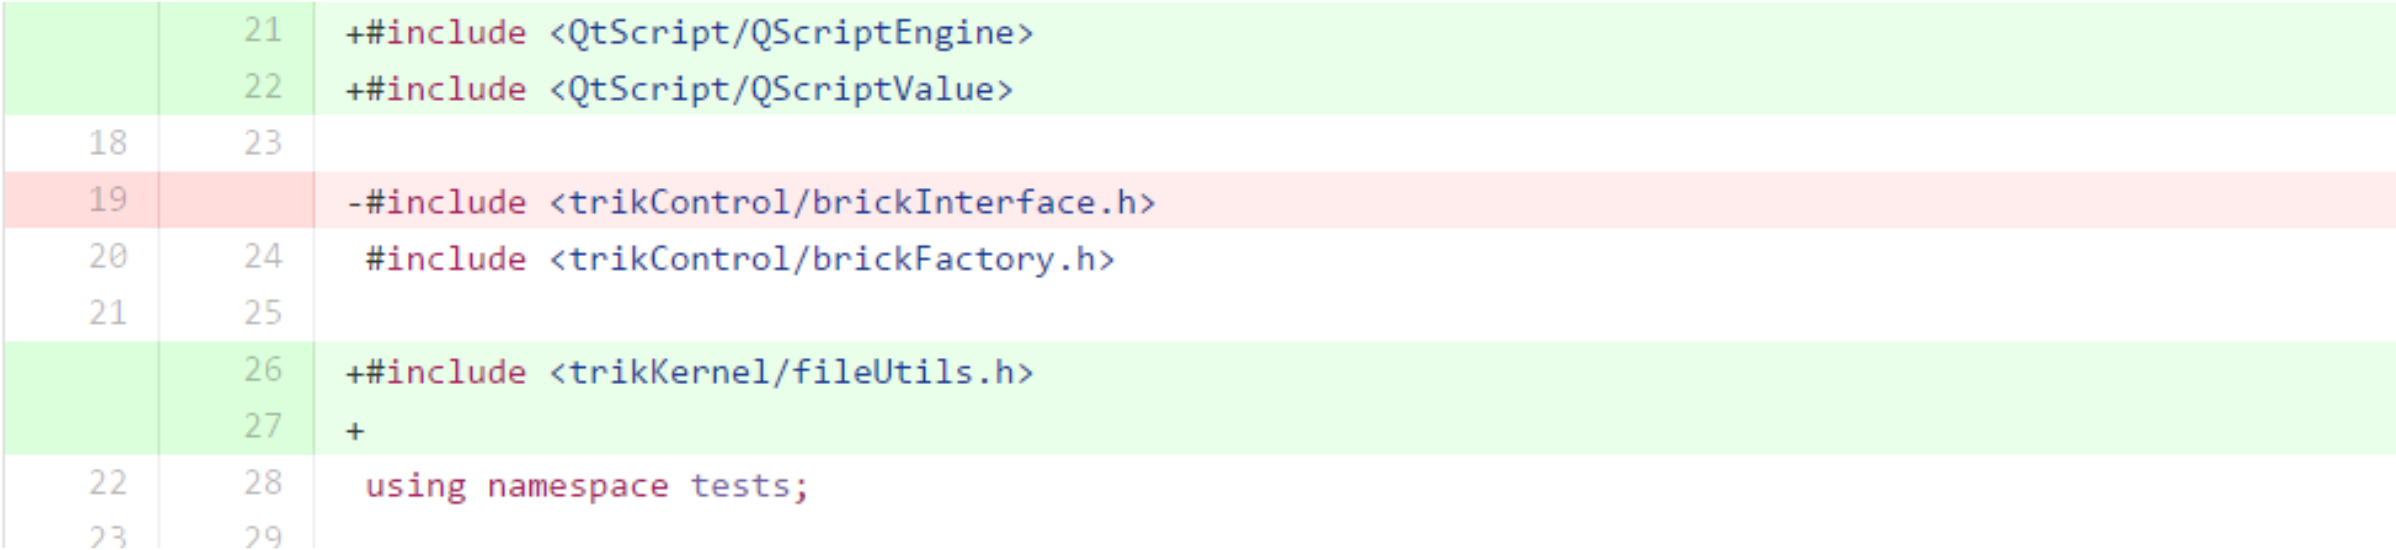
\includegraphics[width=0.9\textwidth]{delta.png}
        \end{center}
    \end{frame}

    \begin{frame}
        \frametitle{Конкретно Git}
        \begin{itemize}
            \item 2005 год, Линус Торвальдс (тот самый)
            \item Консольная утилита, реализованная под все нормальные ОС
            \begin{itemize}
                \item Git for Windows, \url{https://git-scm.com/download/win}
            \end{itemize}
            \item Графические клиенты (много)
            \begin{itemize}
                \item TortoiseGit, \url{https://tortoisegit.org/}
            \end{itemize}
            \item Хостинги репозиториев: GitHub, GitLab, BitBucket, ...
        \end{itemize}
    \end{frame}

    \begin{frame}
        \frametitle{Жизненный цикл файла}
        \begin{center}
            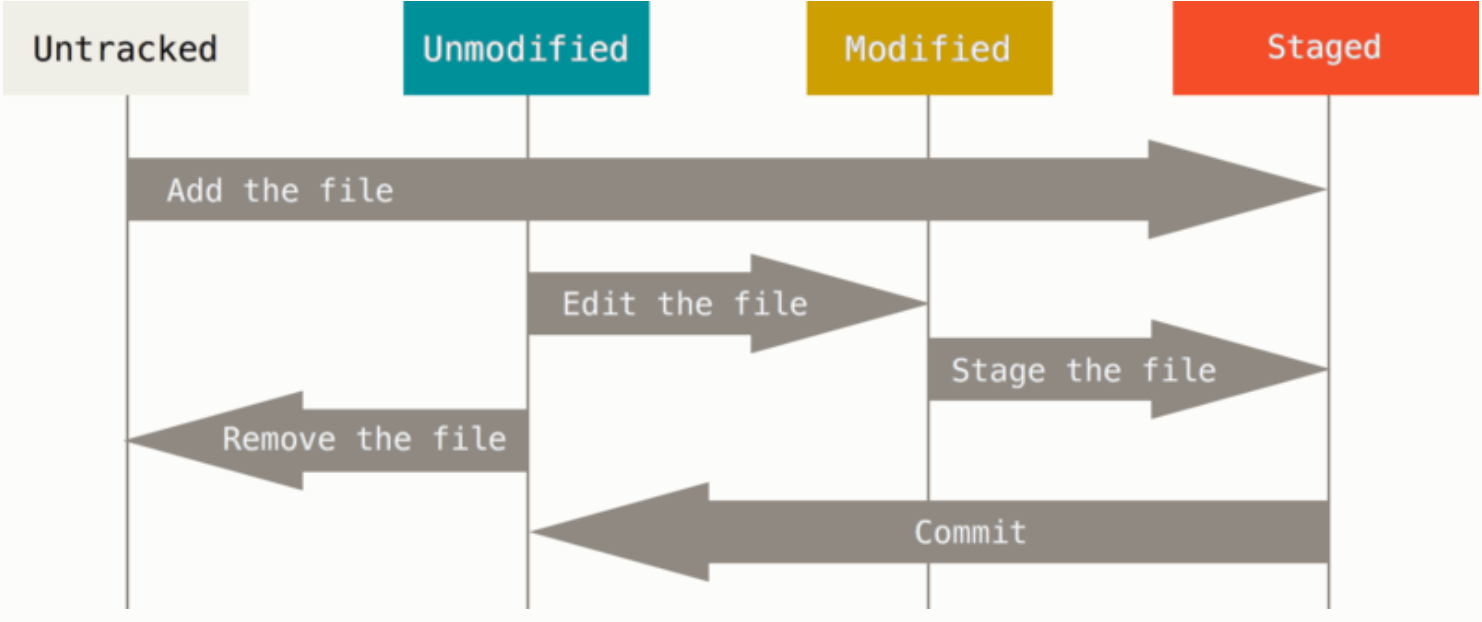
\includegraphics[width=0.8\textwidth]{fileLifeCycle.png}
            \attribution{https://git-scm.com/book/ru}
        \end{center}
    \end{frame}

    \begin{frame}
        \frametitle{Основные команды}
        \begin{itemize}
            \item git add --- добавить новый файл под управление git или добавить изменение к коммиту
            \begin{itemize}
                \item Add... в TortoiseGit
            \end{itemize}
            \item git status --- показать список изменённых/добавленных/удалённых файлов
            \begin{itemize}
                \item Diff в TortoiseGit
            \end{itemize}
            \item git diff --- показать изменения по каждому файлу
            \begin{itemize}
                \item В окне Diff двойным кликом по файлу в TortoiseGit
            \end{itemize}
            \item git commit --- зафиксировать изменения, создав новый коммит
            \begin{itemize}
                \item Git Commit в TortoiseGit
            \end{itemize}
            \item git rm --- удалить файл и удалить его из репозитория
            \begin{itemize}
                \item Delete в TortoiseGit
            \end{itemize}
            \item git log --- просмотреть список коммитов
            \begin{itemize}
                \item Show log в TortoiseGit
            \end{itemize}
            \item git checkout --- откатить изменения в файле или перейти на другую ветку
            \begin{itemize}
                \item Revert... или Switch/Checkout
            \end{itemize}
        \end{itemize}
    \end{frame}

    \begin{frame}
        \frametitle{Демо}
        \begin{itemize}
            \item Надо скачать и поставить Git for Windows и TortoiseGit
            \item Создадим локально репозиторий, научимся коммитить файлы, смотреть историю и откатывать изменения
        \end{itemize}
    \end{frame}

    \begin{frame}[fragile]
        \frametitle{Как всё устроено}
        \begin{minted}{text}
$ git add README test.rb LICENSE
$ git commit -m 'initial commit of my project'
        \end{minted}
        \begin{center}
            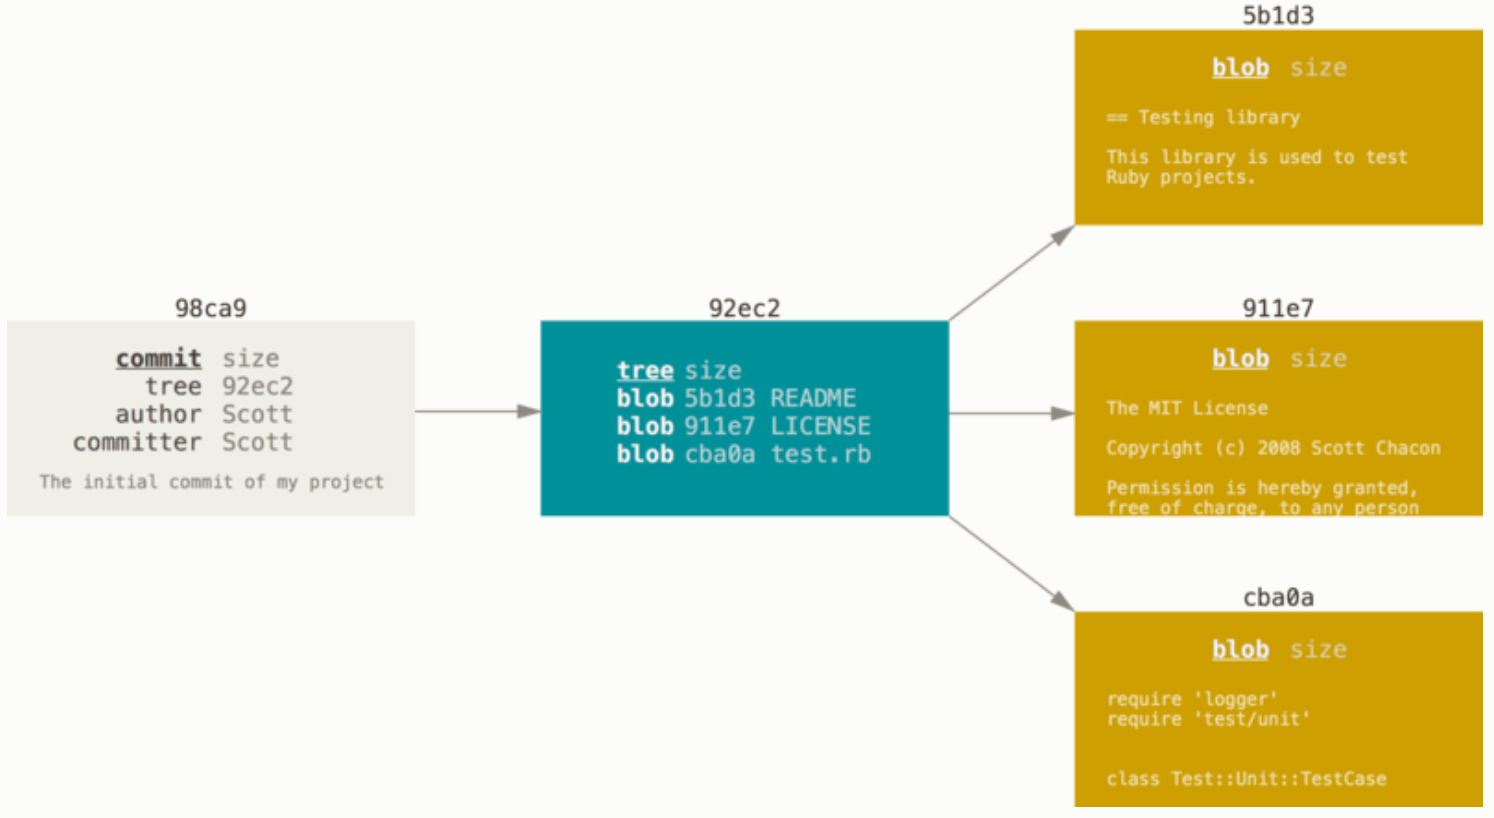
\includegraphics[width=0.8\textwidth]{blobs.png}
            \attribution{https://git-scm.com/book/ru}
        \end{center}
    \end{frame}

    \begin{frame}
        \frametitle{Коммит и его родители}
        \begin{center}
            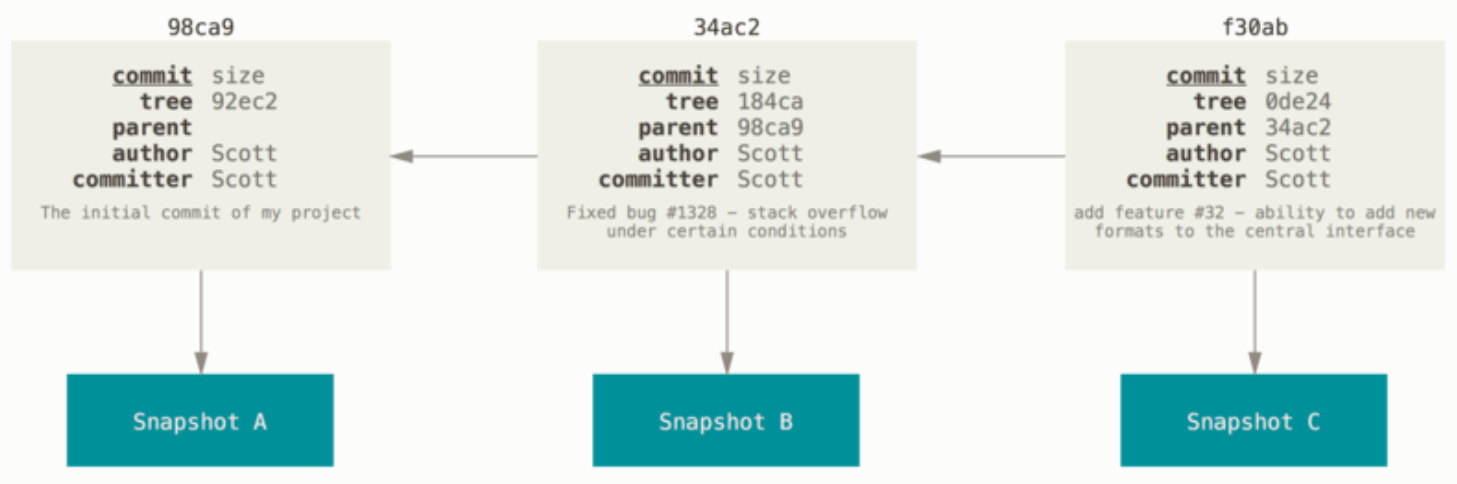
\includegraphics[width=0.8\textwidth]{commits.png}
            \attribution{https://git-scm.com/book/ru}
        \end{center}
    \end{frame}

    \begin{frame}
        \frametitle{Ветки}
        \begin{center}
            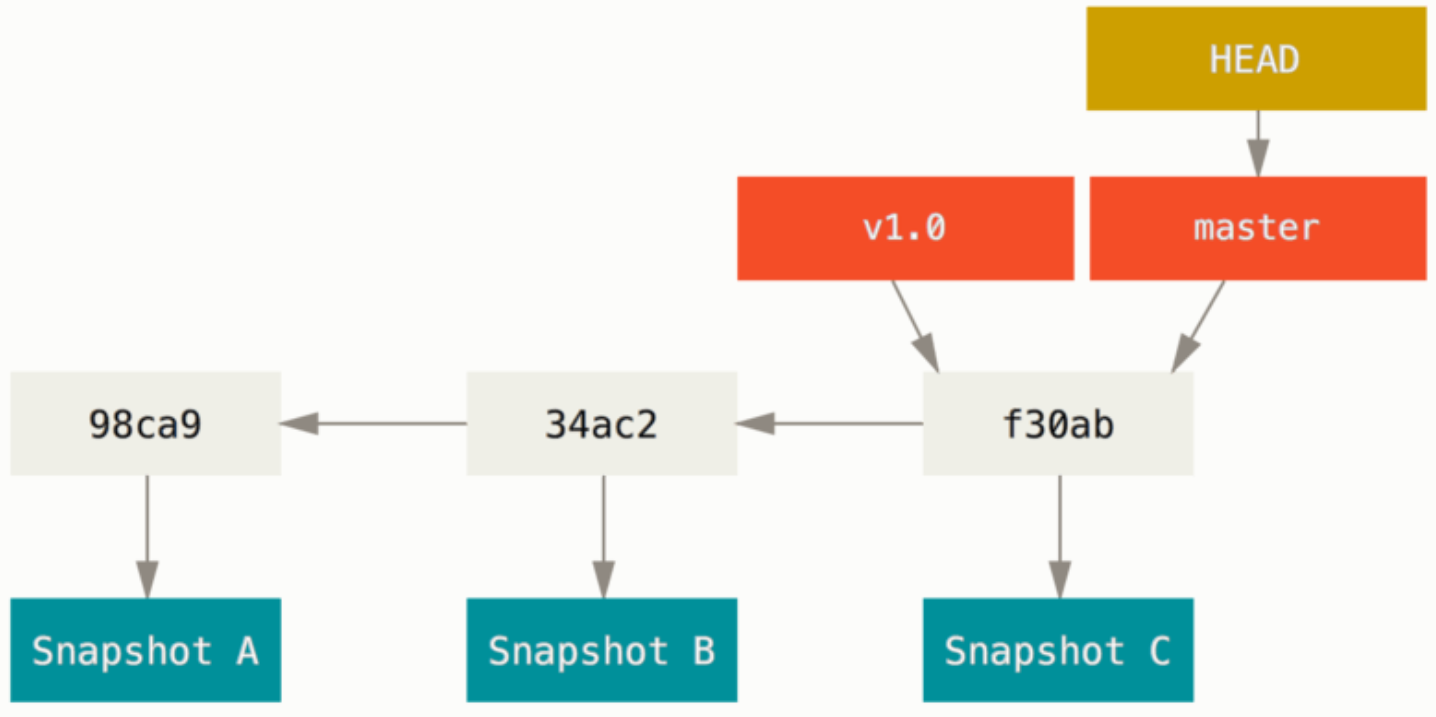
\includegraphics[width=0.8\textwidth]{branches.png}
            \attribution{https://git-scm.com/book/ru}
        \end{center}
    \end{frame}

    \begin{frame}[fragile]
        \frametitle{Создание ветки}
        \begin{minted}{text}
$ git branch testing
        \end{minted}
        \begin{center}
            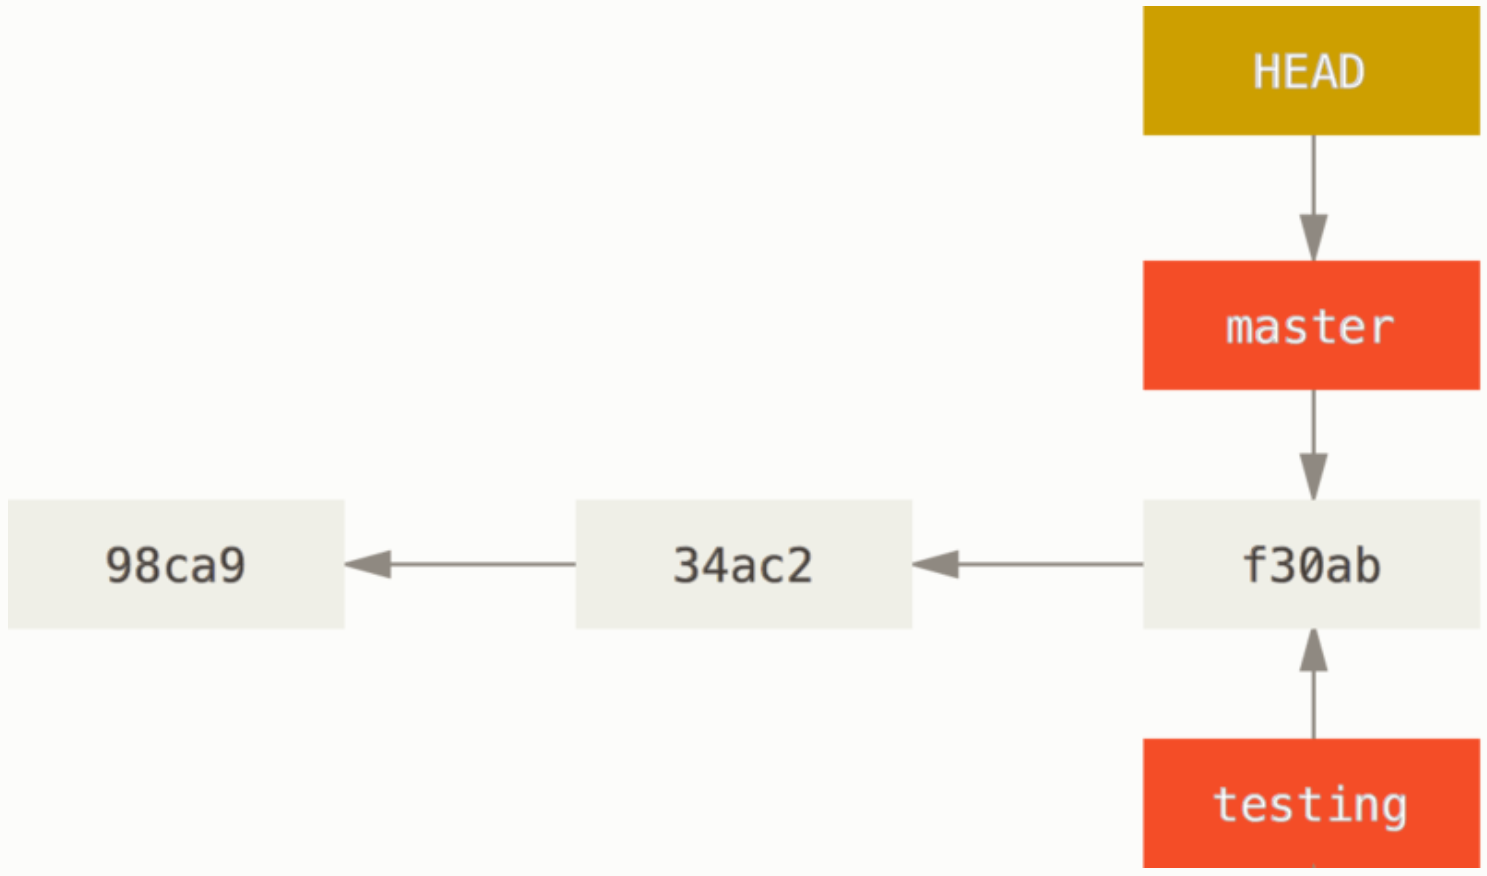
\includegraphics[width=0.8\textwidth]{creatingBranch.png}
            \attribution{https://git-scm.com/book/ru}
        \end{center}
    \end{frame}

    \begin{frame}[fragile]
        \frametitle{Переключение ветки}
        \begin{minted}{text}
$ git checkout testing
        \end{minted}
        \begin{center}
            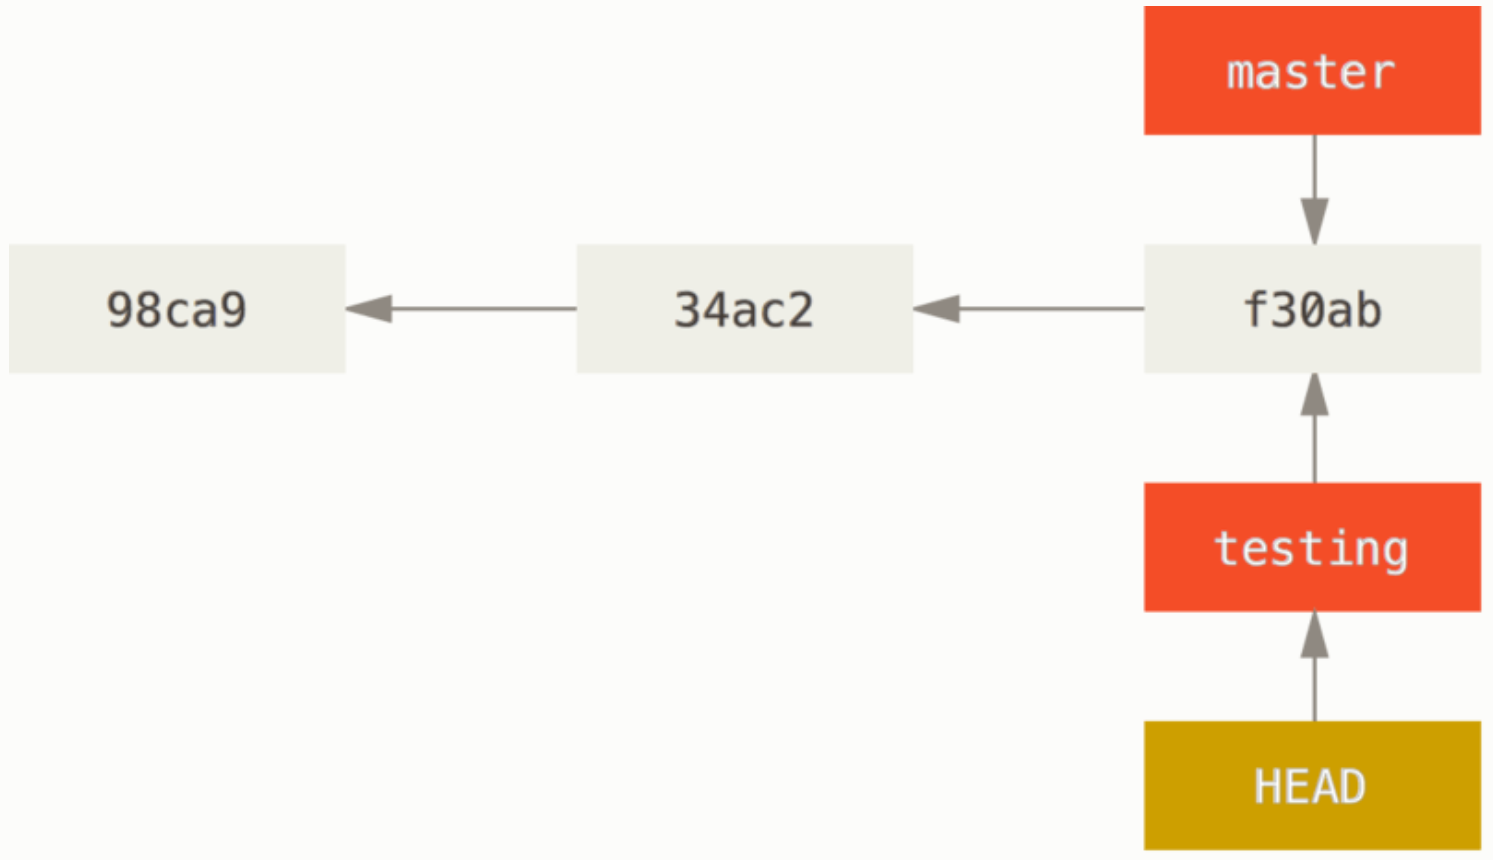
\includegraphics[width=0.8\textwidth]{checkout.png}
            \attribution{https://git-scm.com/book/ru}
        \end{center}
    \end{frame}

    \begin{frame}[fragile]
        \frametitle{Новый коммит}
        \begin{minted}{text}
<Что-то поделали с файлами в рабочей копии>
$ git add <изменения, которые хотим коммитить>
$ git commit -m 'made a change'
        \end{minted}
        \begin{center}
            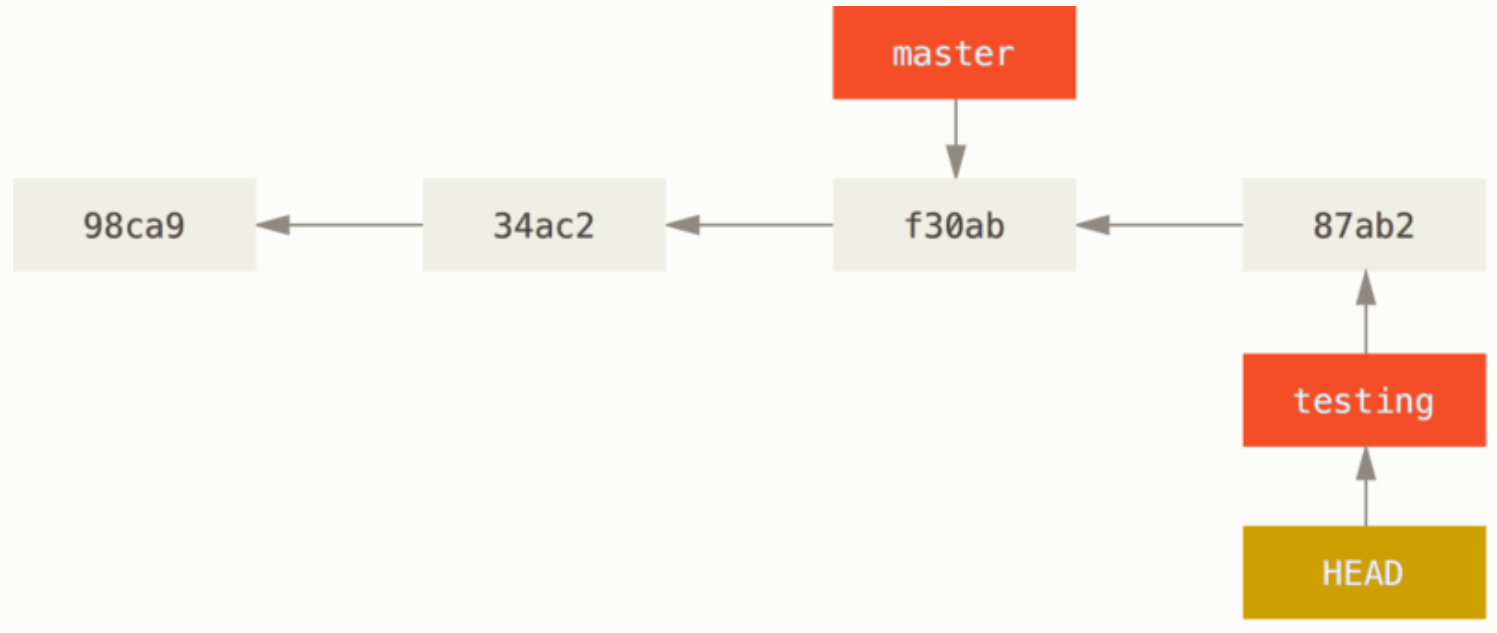
\includegraphics[width=0.8\textwidth]{newCommit.png}
            \attribution{https://git-scm.com/book/ru}
        \end{center}
    \end{frame}

    \begin{frame}[fragile]
        \frametitle{Переключимся на master}
        \begin{minted}{text}
$ git checkout master
        \end{minted}
        \begin{center}
            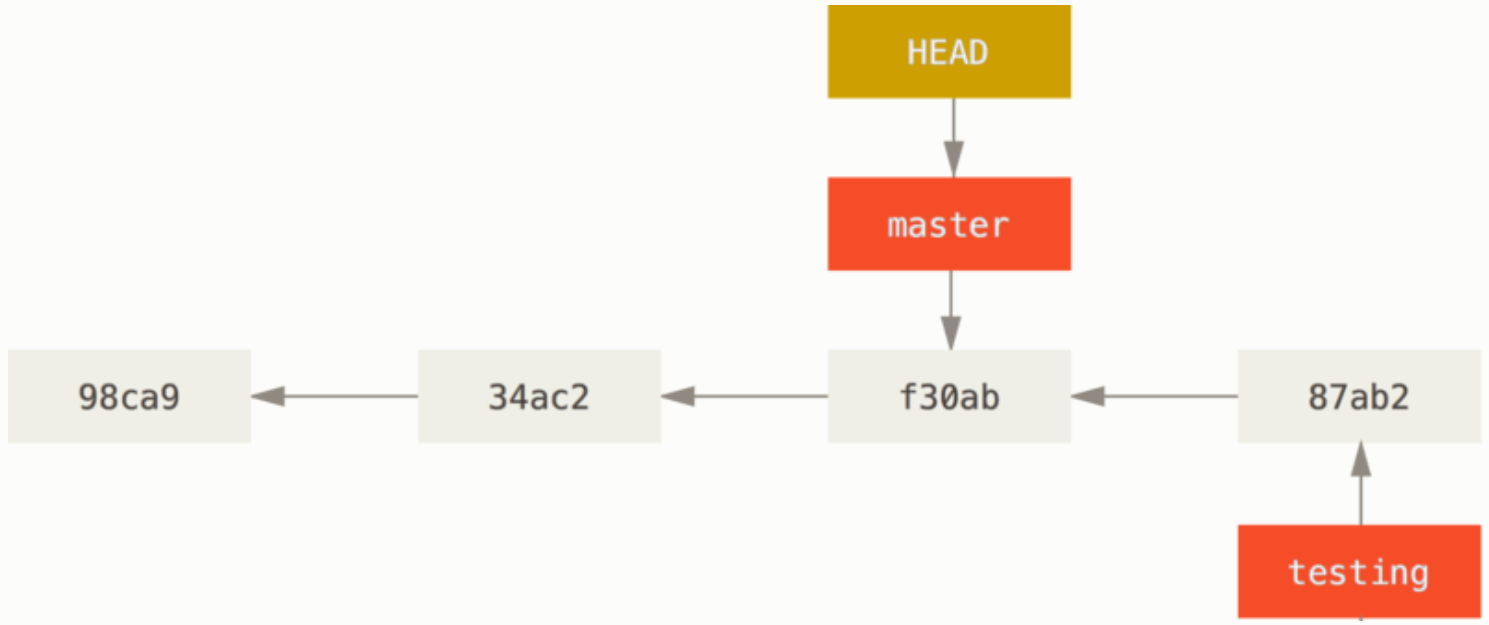
\includegraphics[width=0.8\textwidth]{checkoutToMaster.png}
            \attribution{https://git-scm.com/book/ru}
        \end{center}
    \end{frame}

    \begin{frame}[fragile]
        \frametitle{Сделаем новый коммит там}
        \begin{minted}{text}
<Что-то поделали с файлами в рабочей копии>
$ git add <изменения, которые хотим коммитить>
$ git commit -m 'made other changes'
        \end{minted}
        \begin{center}
            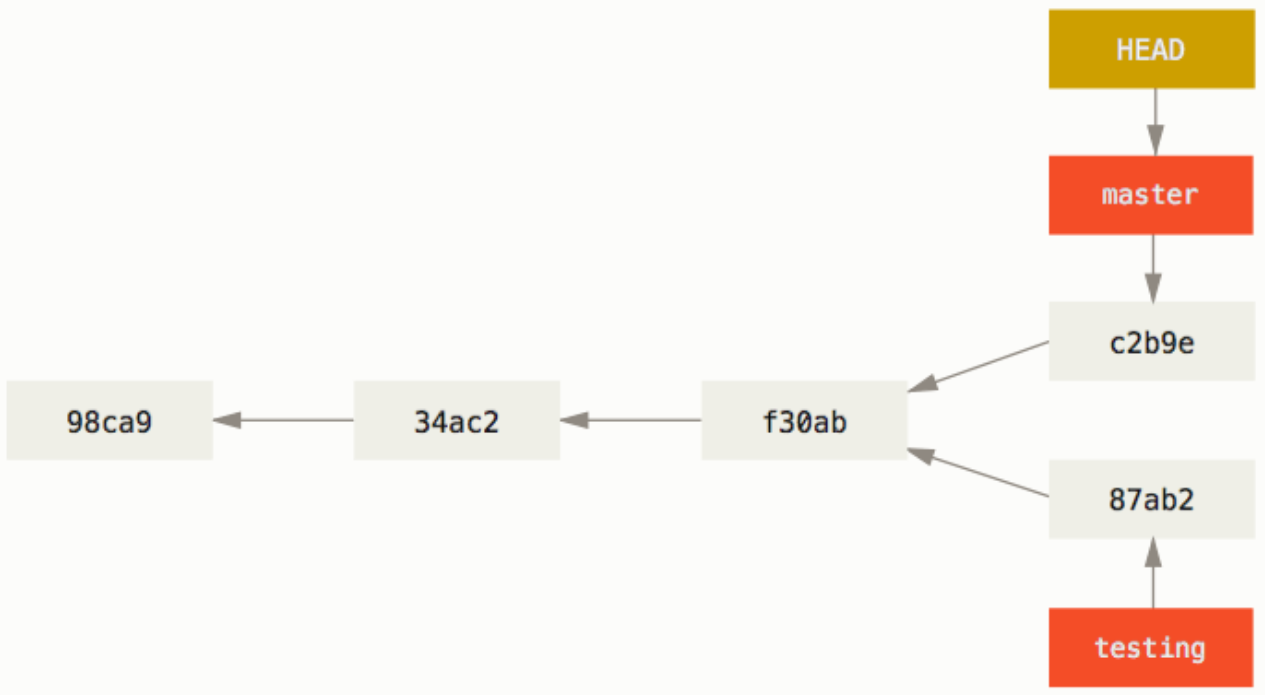
\includegraphics[width=0.8\textwidth]{newCommitToMaster.png}
            \attribution{https://git-scm.com/book/ru}
        \end{center}
    \end{frame}

    \begin{frame}[fragile]
        \frametitle{Слияние веток}
        \begin{minted}{text}
$ git checkout master
Switched to branch 'master'
$ git merge testing
Merge made by the 'recursive' strategy.
index.html |    1 +
1 file changed, 1 insertion(+)
        \end{minted}
        \begin{center}
            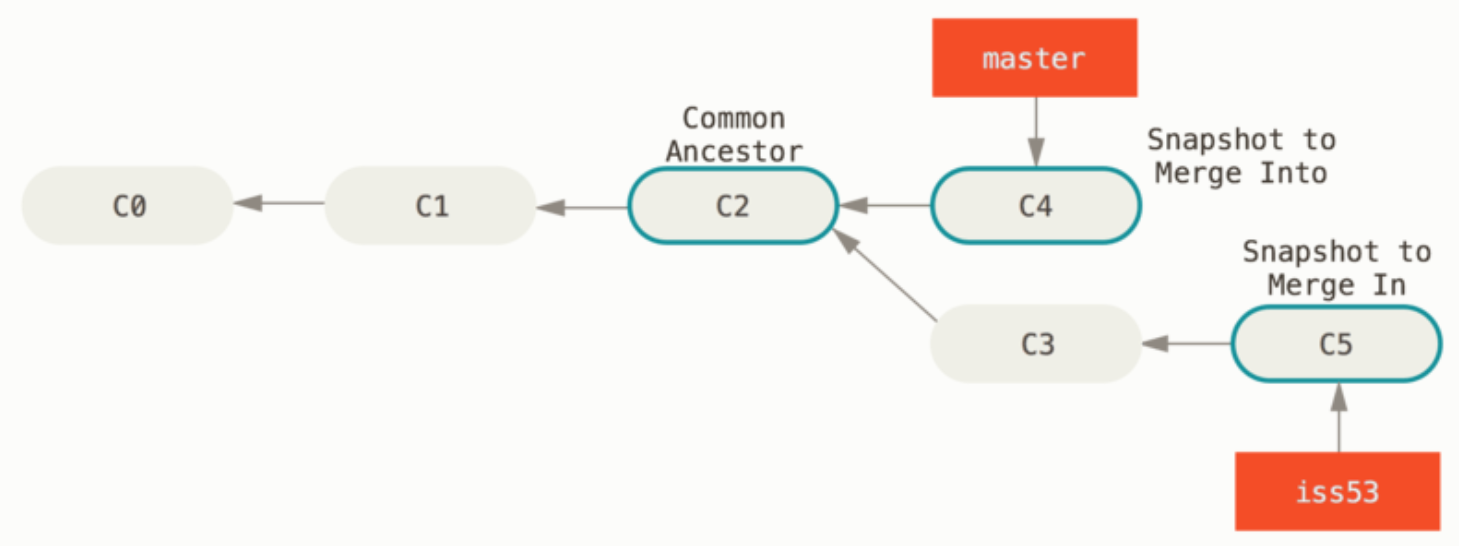
\includegraphics[width=0.8\textwidth]{merge.png}
            \attribution{https://git-scm.com/book/ru}
        \end{center}
    \end{frame}

    \begin{frame}
        \frametitle{Результат}
        \begin{center}
            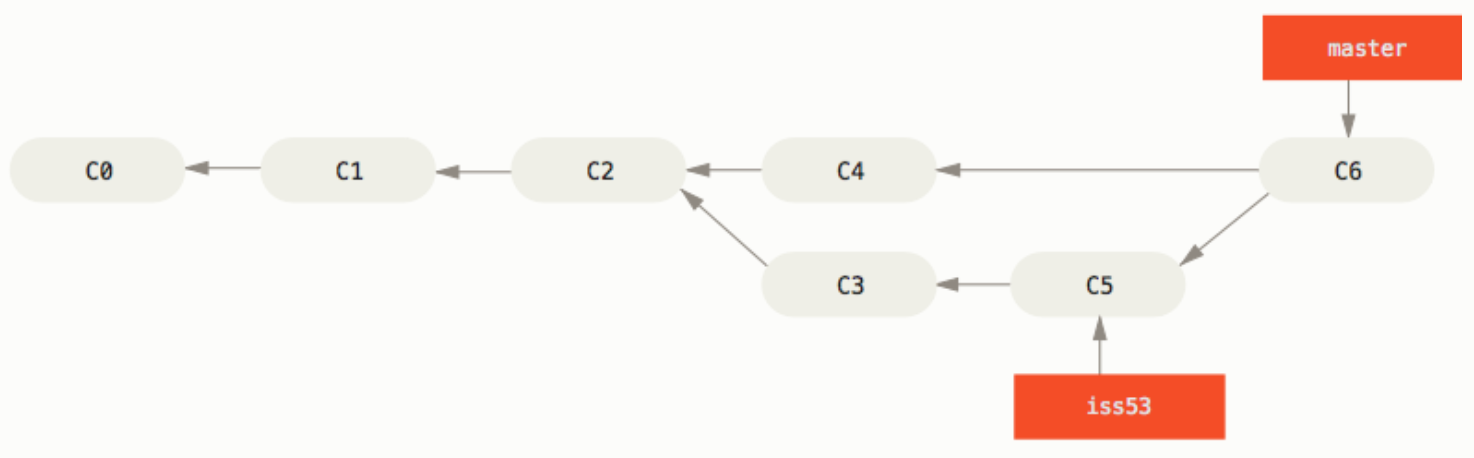
\includegraphics[width=0.8\textwidth]{mergeResult.png}
            \attribution{https://git-scm.com/book/ru}
        \end{center}
    \end{frame}

    \begin{frame}
        \frametitle{Конфликты}
        \begin{center}
            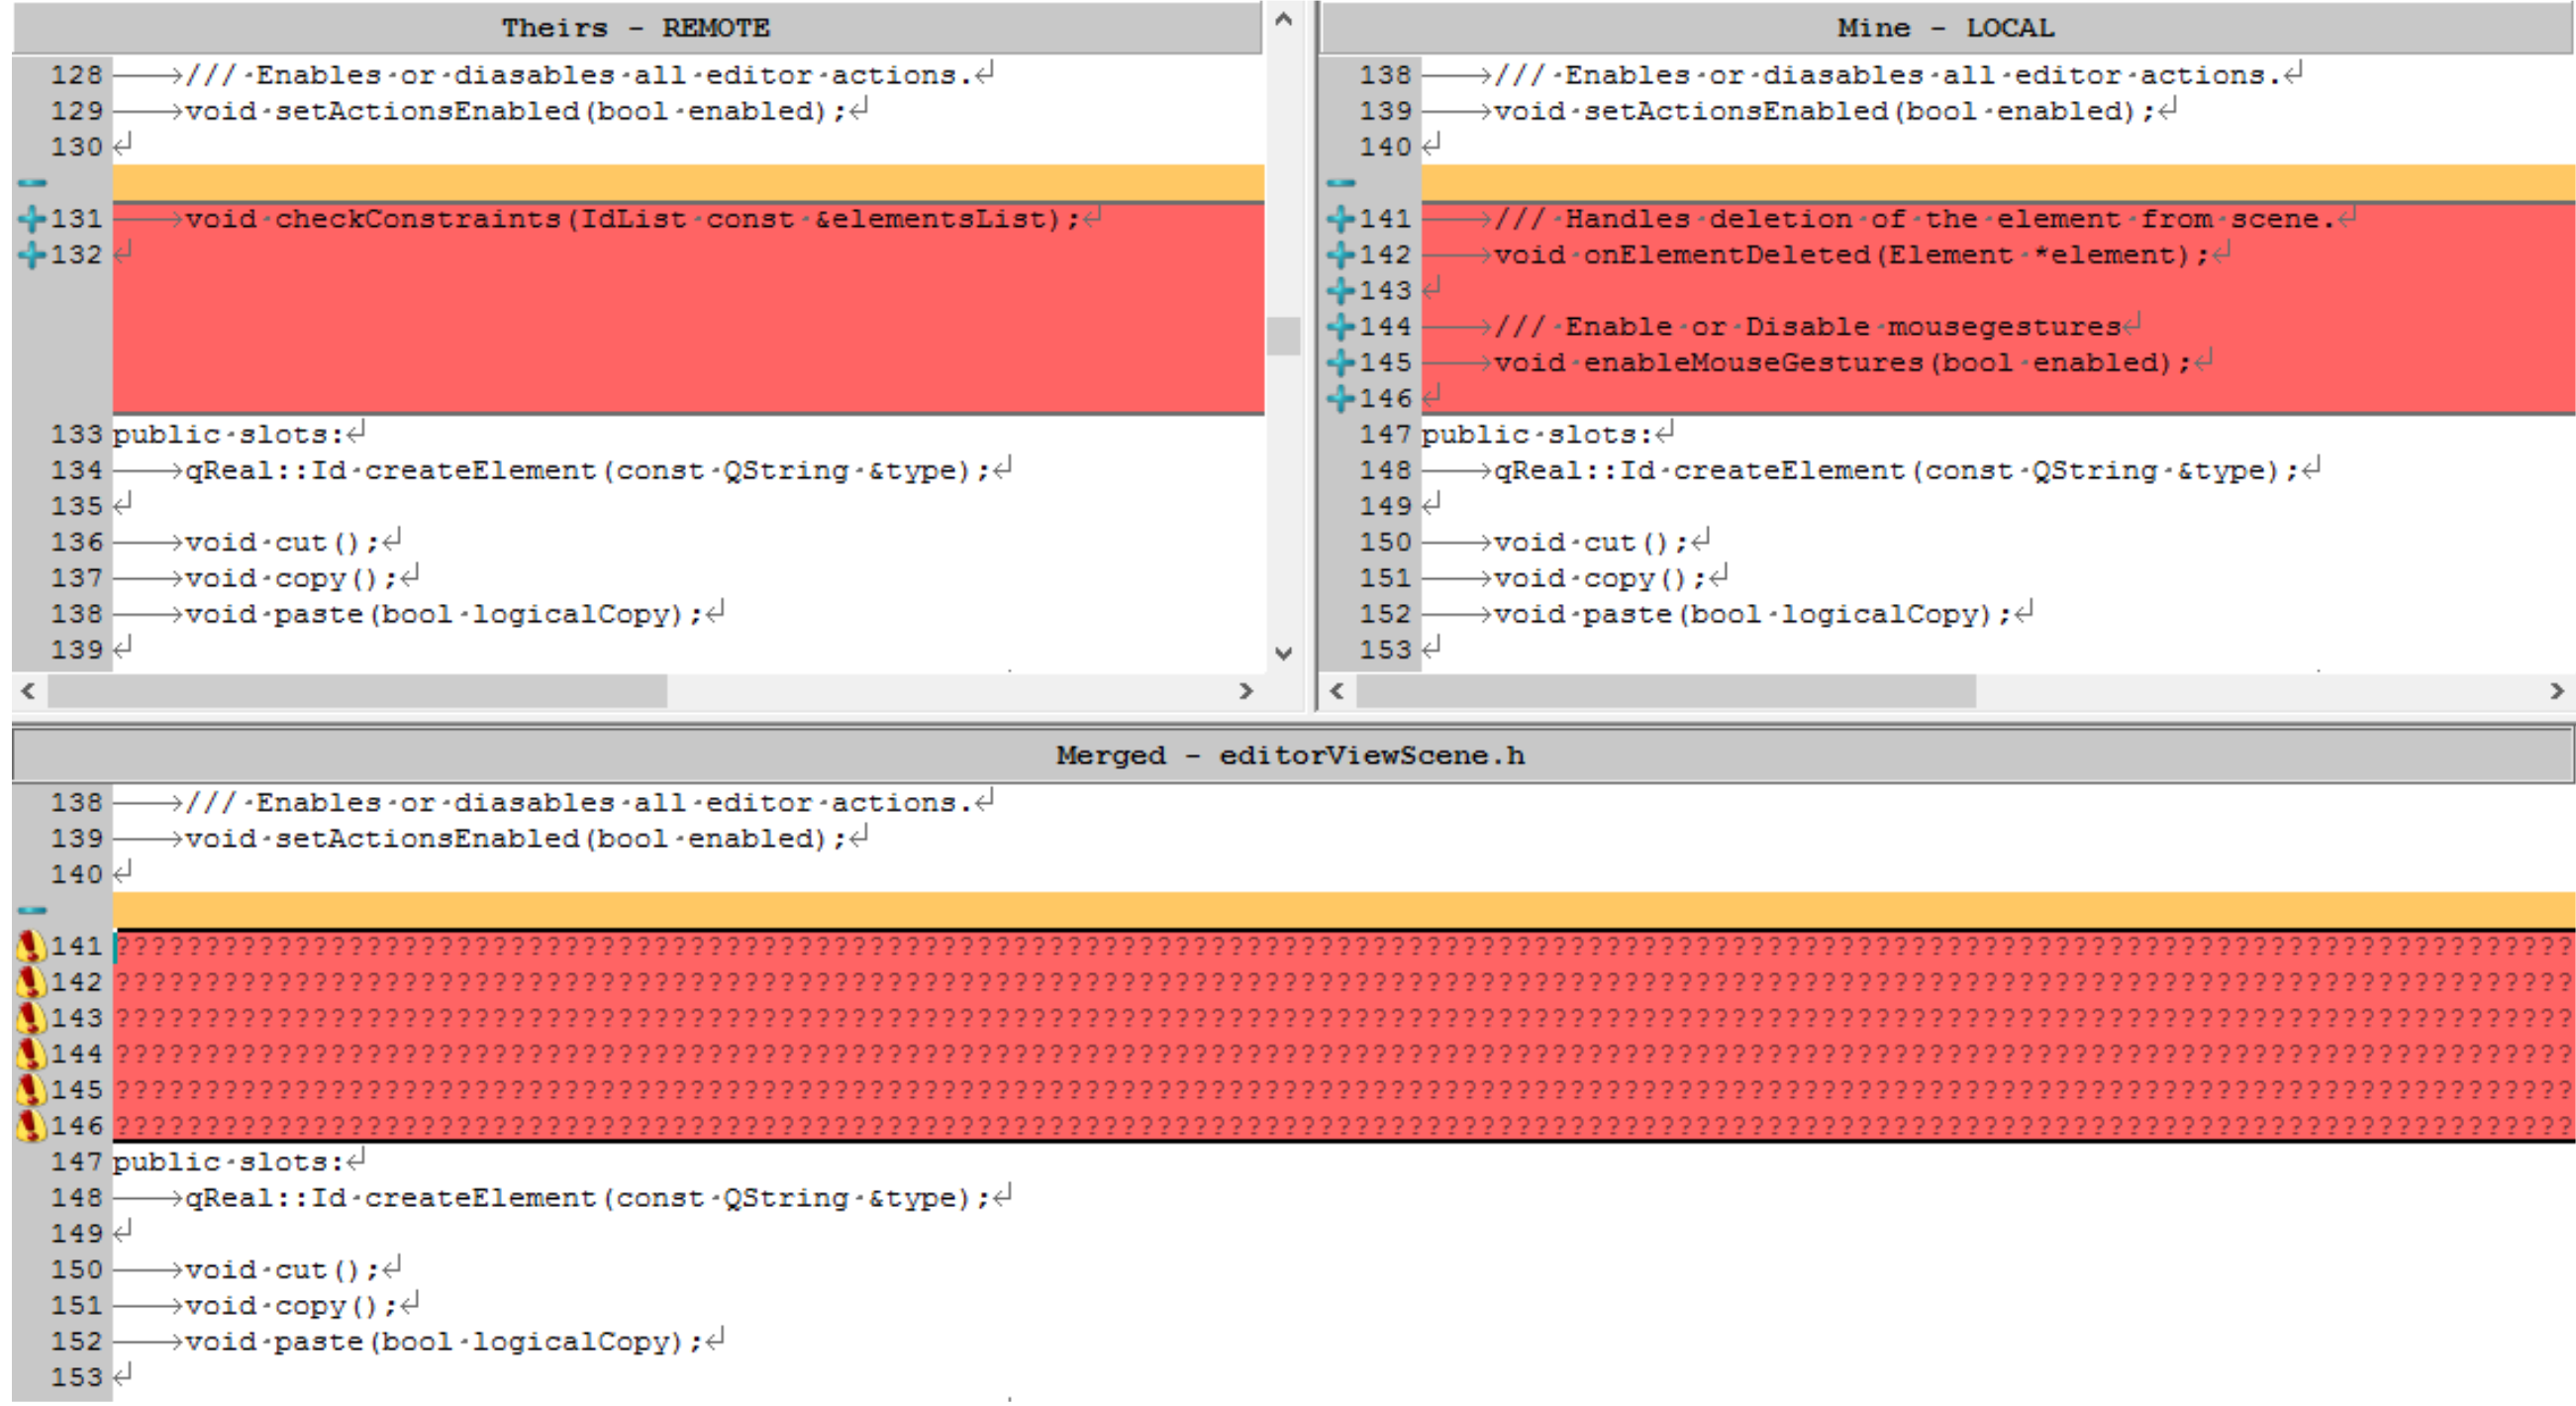
\includegraphics[width=0.95\textwidth]{conflicts.png}
        \end{center}
    \end{frame}

    \begin{frame}
        \frametitle{Конфликты в коде}
        \begin{center}
            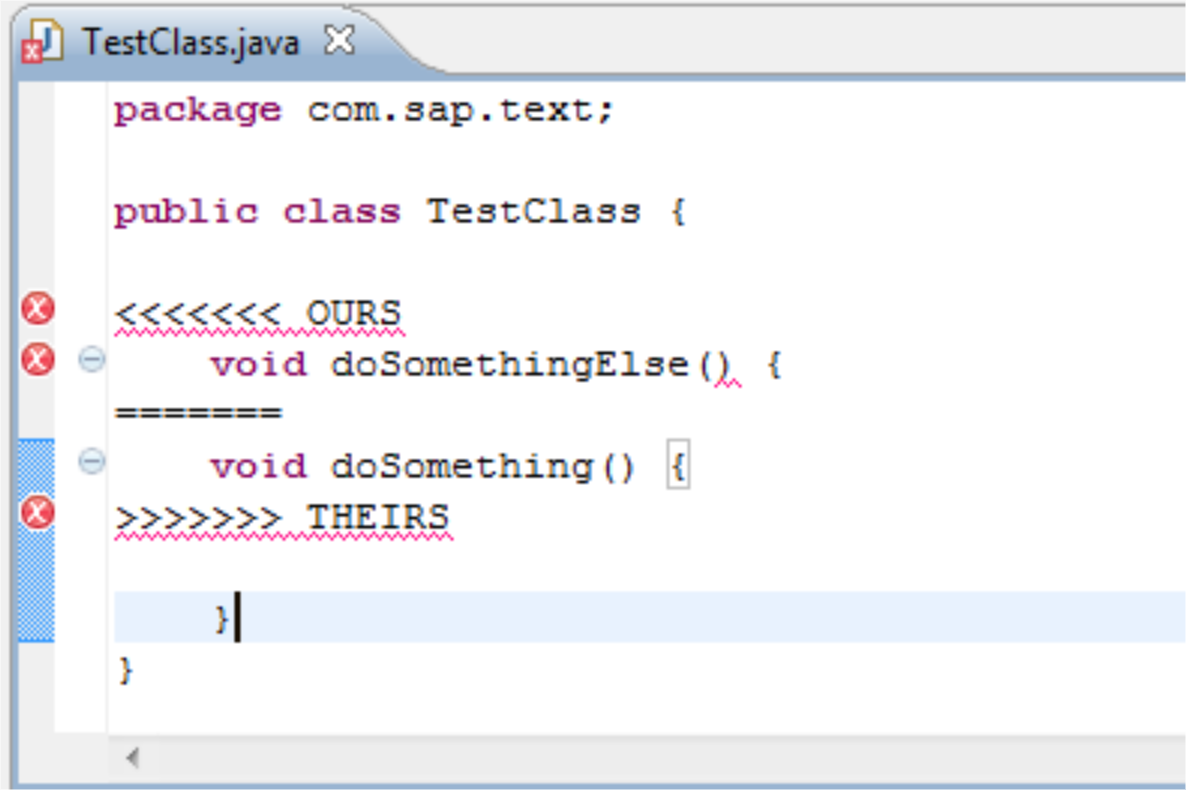
\includegraphics[width=0.5\textwidth]{conflictsInCode.png}
        \end{center}
    \end{frame}

    \begin{frame}
        \frametitle{Удалённые репозитории}
        \begin{columns}
            \begin{column}{0.4\textwidth}
                \begin{itemize}
                    \item git clone
                    \item git remote
                    \item git push
                    \item git fetch
                    \item git pull
                    \item Соответствующие команды в окне Git Sync... в TortoiseGit
                \end{itemize}
            \end{column}
            \begin{column}{0.6\textwidth}
                \begin{center}
                    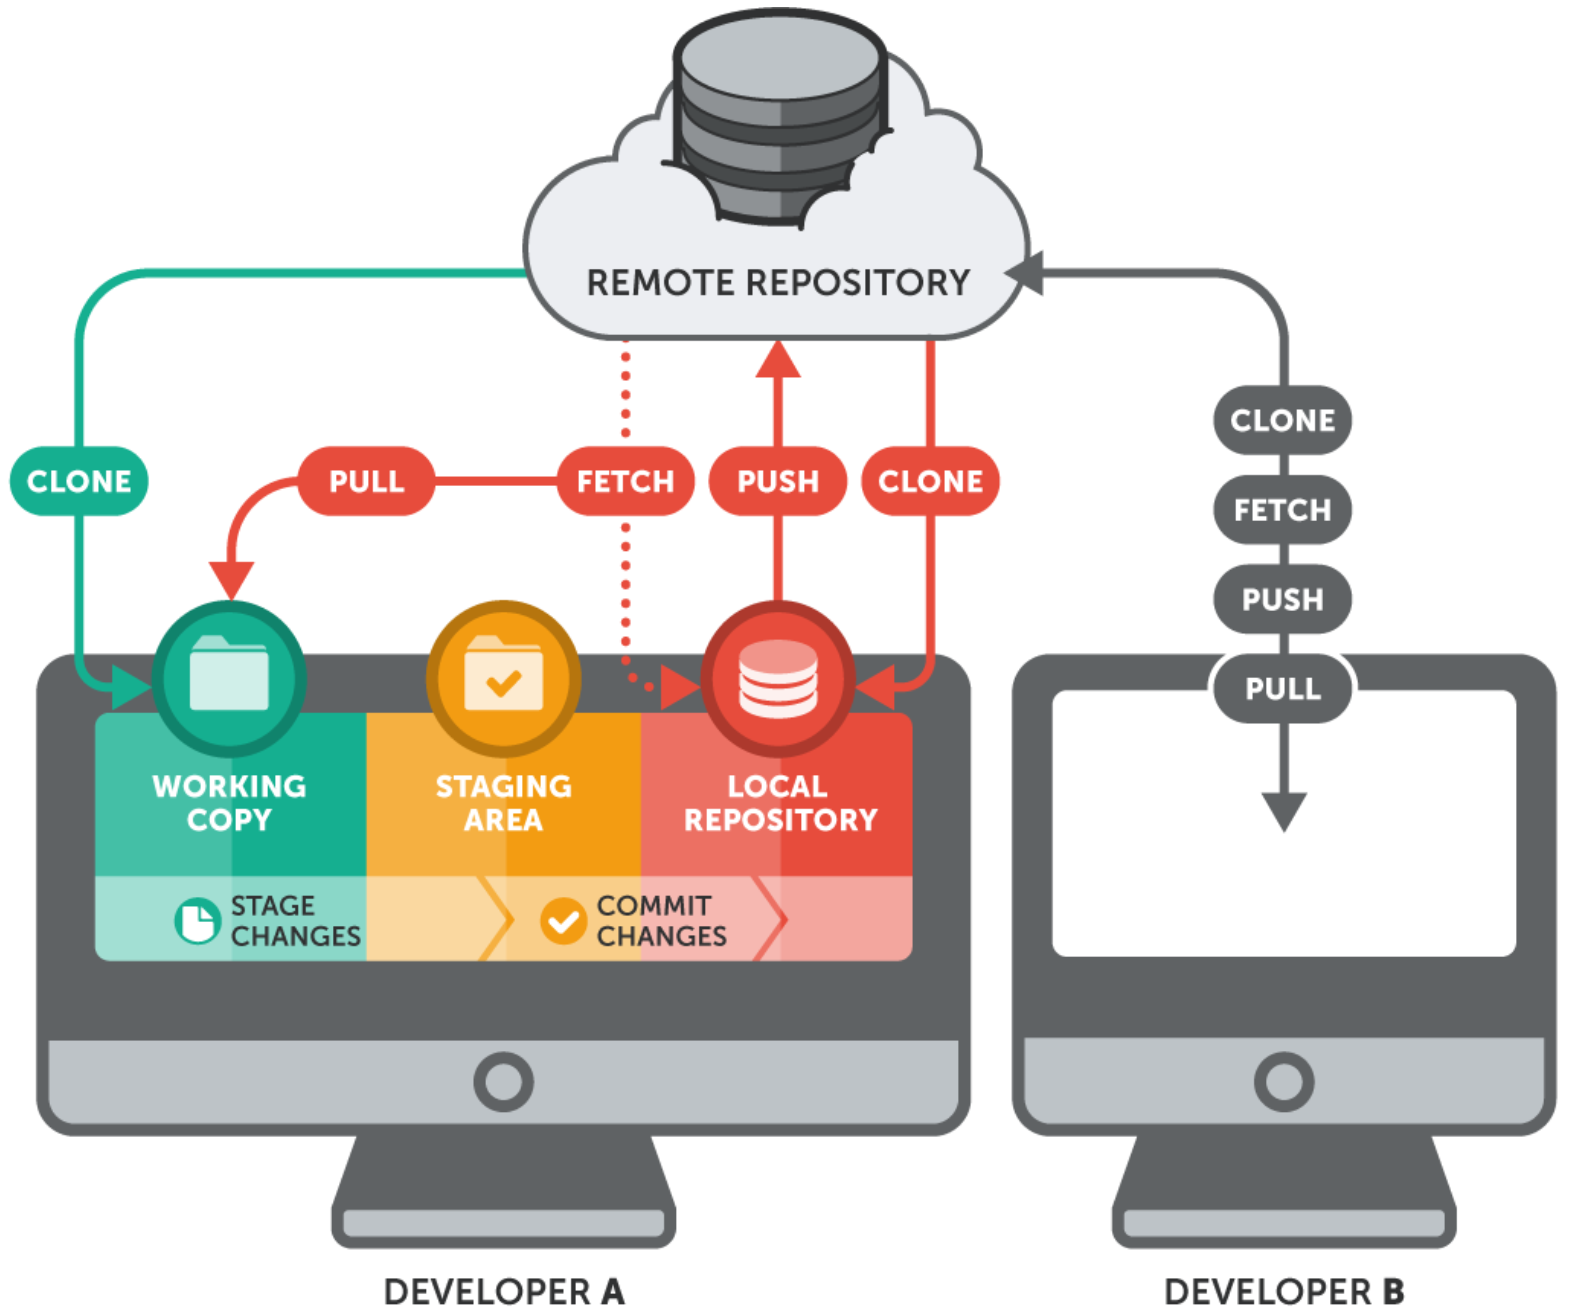
\includegraphics[width=0.95\textwidth]{remoteRepos.png}
                    \attribution{https://www.git-tower.com/learn/git/ebook/en}
                \end{center}
            \end{column}
        \end{columns}
    \end{frame}

    \begin{frame}
        \frametitle{Демо}
        \begin{itemize}
            \item Регистрируемся на GitHub
            \item Создаём репозиторий прямо на GitHub
            \item Клоним его себе
            \item Отводим ветку под домашку
            \item Делаем её там
            \item Коммитим/пушим
            \item Делаем пуллреквест в main
        \end{itemize}
    \end{frame}

    \begin{frame}
        \frametitle{Процесс работы}
        \begin{footnotesize}
            \begin{itemize}
                \item Программист хочет сделать новую фичу
                \item Отводит себе ветку от main-а
                \item Реализует там фичу
                \item Тестит и рефакторит её, когда считает, что она готова, делает пуллреквест
                \item Пока пуллреквест ревьюят, программист делает новую фичу (опять-таки, отведя новую ветку от main-а)
                \item По пуллреквесту появляются замечания, программист переключается на ветку пуллреквеста и правит там замечания
                \item Когда поправил, коммитит и пушит исправления, они автоматом добавляются в пуллреквест
                \item Просит ревьюеров, чтобы они посмотрели фиксы
                \item Переключается обратно на свою рабочую ветку и продолжает писать код, возможно, делая ещё пуллреквесты 
                \item Цикл повторяется до тех пор, пока пуллреквест не принимают
                \item Программист удаляет ветку с фичей, когда она замерджена
            \end{itemize}
        \end{footnotesize}
    \end{frame}

    \begin{frame}
        \frametitle{То же, но с домашкой}
        \begin{itemize}
            \item Хотите сделать новую задачу
            \item Отводите себе ветку от main-а
            \begin{itemize}
                \item Create Branch..., Base On --- main
                \item Вводите адекватное имя ветки (например, номер или название задачи)
            \end{itemize}
            \item Создаёте \emph{прямо там} проект, делаете задачу
            \item Коммитите, сколько хотите
            \begin{itemize}
                \item После каждого значимого продвижения
                \item Git Commit -> имя вашей ветки (проверьте, что не main)
                \item Вводим в message \emph{внятное} описание изменений
            \end{itemize}
        \end{itemize}
    \end{frame}

    \begin{frame}
        \frametitle{То же, но с домашкой (2)}
        \begin{itemize}
            \item Когда считаете, что задача готова, пушите её на GitHub
            \begin{itemize}
                \item Git Sync -> Push
            \end{itemize}
            \item Идёте на GitHub, делаете пуллреквест
            \begin{itemize}
                \item Выбираете ветку в ``Branch:''
                \item Жмёте на Pull request
                \item Вводите внятное описание пуллреквеста
                \item Жмёте на Create pull request
            \end{itemize}
            \item Ссылку на то, что получилось, выкладываете на Blackboard
            \begin{itemize}
                \item Список всех пуллреквестов можно посмотреть во вкладке Pull requests на GitHub
            \end{itemize}
            \item Ждёте, пока я прокомментирую решение
        \end{itemize}
    \end{frame}

    \begin{frame}
        \frametitle{То же, но с домашкой (3)}
        \begin{itemize}
            \item В это время можно заняться следующей задачей
            \begin{itemize}
                \item Create Branch..., Base On --- main
            \end{itemize}
            \item Получаете ревью на GitHub, исправляете замечания
            \begin{itemize}
                \item Переключаетесь на исходную ветку
                \begin{itemize}
                    \item Коммитите текущие изменения в рабочей копии
                    \item Switch/Checkout -> исходная ветка
                \end{itemize}
                \item Исправляете, коммитя сколько хотите
                \item Коммитите исправления
                \item Пушите на GitHub
            \end{itemize}
            \item Проверяете, что всё ок, в пуллреквестах на GitHub
            \begin{itemize}
                \item Пуллреквест пересоздавать не надо, пуллреквест открывается от ветки, а не от коммита
            \end{itemize}
            \item Когда задача принята, мерджите пуллреквест на GitHub и удаляете ветку
        \end{itemize}
    \end{frame}

    \begin{frame}
        \frametitle{Что надо выкладывать}
        \begin{itemize}
            \item .c, .h-файлы
            \item Проектные файлы:
            \begin{itemize}
                \item Visual Studio: .vcxproj, .sln
                \item CLion: всё содержимое папки .idea, кроме workspace.xml и tasks.xml
            \end{itemize}
            \item Текстовые файлы и прочие ресурсы, которые используются в тестах или во время работы программы
        \end{itemize}
    \end{frame}

    \begin{frame}
        \frametitle{Что не надо выкладывать}
        \begin{itemize}
            \item Бинарные файлы: .exe, .dll, бинарники под линуксом
            \begin{itemize}
                \item Включите себе отображение расширений файлов
            \end{itemize}
            \item Промежуточные результаты компиляции: .o, .obj, ...
            \item Скрытую папку .vs в Visual Studio
            \begin{itemize}
                \item Включите себе отображение скрытых файлов
            \end{itemize}
        \end{itemize}
        .gitignore:
        \begin{itemize}
            \item \url{https://git-scm.com/docs/gitignore}
            \item \url{https://github.com/github/gitignore}
        \end{itemize}
    \end{frame}

    \begin{frame}
        \frametitle{Хорошие практики}
        \begin{itemize}
            \item При первом коммите попросят имя и Email, аккуратно заполняем
            \begin{itemize}
                \item Желательно, чтобы они совпадали с именем аккаунта и почтой, с которой регались на GitHub
            \end{itemize}
            \item Коммитим только то, что нужно, чтобы получить в чистую папку и собрать проект
            \item Всегда пишем адекватные комментарии к коммитам
            \item Коммитим как можно чаще
            \item Один коммит --- одна функциональность
            \begin{itemize}
                \item Сделали что-то, хоть немного напоминающее осмысленное -> коммит
            \end{itemize}
        \end{itemize}
    \end{frame}

    \begin{frame}
        \frametitle{Хорошие практики (2)}
        \begin{itemize}
            \item Коммит не должен содержать в себе файлы, не относящиеся к изменениям
            \begin{itemize}
                \item .gitignore
            \end{itemize}
            \item Коммит не должен добавлять/убирать пустые строки, менять пробелы на табы и т.д., если это не суть коммита
            \item Стиль исходного кода и отступов должен совпадать с текстом вокруг
        \end{itemize}
        \begin{center}
            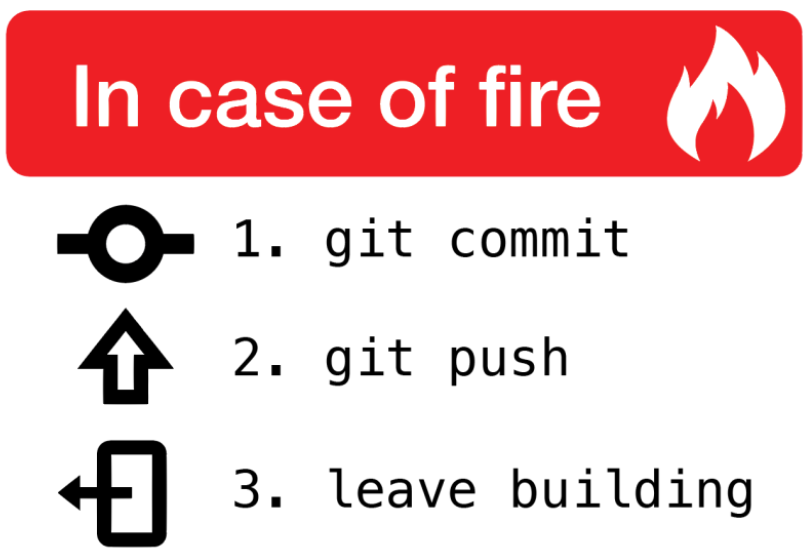
\includegraphics[width=0.4\textwidth]{inCaseOfFire.png}
        \end{center}
    \end{frame}

\end{document}

